% Nier_ANLP -- SemEval-2026 Task 6 (CLARITY) course report, VERSION 2 (figures re-drawn by clarity/paper_figures.py; text identical to main.tex).
% Built on the official ACL template (acl_latex_template.tex, acl-org/acl-style-files @ d5adc82);
% acl.sty and acl_natbib.bst are unmodified copies. Build: bash build.sh
\documentclass[11pt]{article}

% "final": the camera-ready (non-anonymous) version, as the template's comment describes.
\usepackage[final]{acl}

% Standard package includes (as in the official template)
\usepackage{times}
\usepackage{latexsym}
\usepackage[T1]{fontenc}
\usepackage[utf8]{inputenc}
\usepackage{microtype}
\usepackage{inconsolata}
\usepackage{graphicx}

% Content packages (no layout changes)
\usepackage{amsmath}
\usepackage{amssymb}
\usepackage{booktabs}

% Shared notation (owned by the orchestrator)
\newcommand{\Stwo}{S2}
\newcommand{\Sone}{S1}
\newcommand{\pmsd}[2]{#1\,{\scriptsize$\pm$\,#2}}

% Figures of this version (v2: publication figures from clarity/paper_figures.py)
% Version-specific figures. main.tex (v1) inputs figs_v1.tex; main_v2.tex inputs figs_v2.tex.
% The sections call \FigureEncSeeds (column width, in sec:encoder) and \FigureLLM (text width, in sec:llm).
% v2: the same numbers, re-drawn for print by clarity/paper_figures.py (vector PDF, serif type).

\newcommand{\FigureEncSeeds}{%
\begin{figure}[t]
\centering
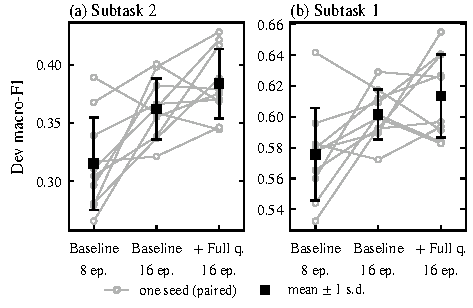
\includegraphics[width=\columnwidth]{figures/v2/fig_deberta_seeds.pdf}
\caption{Single DeBERTa-v3-large models on dev for the three configurations: (a)~\Stwo{} multi-reference macro-F1, (b)~\Sone{} macro-F1. Open circles joined by thin lines are individual seeds, paired across configurations; filled squares are the mean over the 10 seeds, with error bars of $\pm 1$ standard deviation.}
\label{fig:enc-seeds}
\end{figure}}

\newcommand{\FigureLLM}{%
\begin{figure*}[t]
\centering
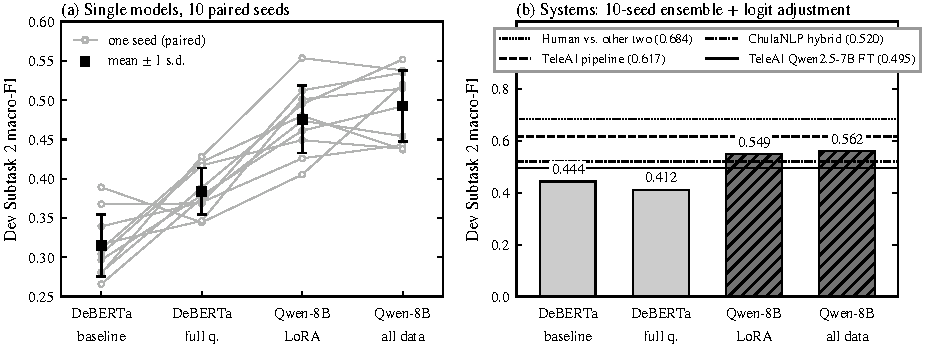
\includegraphics[width=\textwidth]{figures/v2/fig_qwen_vs_deberta.pdf}
\caption{Dev \Stwo{} multi-reference macro-F1 of the DeBERTa-v3-large baseline, DeBERTa with the full question and 16 epochs, Qwen3-8B-Base with LoRA on the same input (3 epochs), and Qwen trained on all of train. (a)~Single models on 10 paired seeds: open circles joined by thin lines are individual seeds; filled squares are means with $\pm 1$ standard deviation. (b)~The corresponding 10-seed systems (ensemble + logit adjustment, $\tau$ by nested CV; bar height is the mean over 10 CV splits), with published dev results as horizontal lines: TeleAI's multi-call pipeline (0.617) and fine-tuned Qwen2.5-7B (0.495) \citep{shi-etal-2026-teleai}, ChulaNLP's DeBERTa top-5 + Kimi-K2 pipeline (0.52) \citep{peerachaidecho-rutherford-2026-chulanlp}, and a human annotator scored against the other two (0.684).}
\label{fig:llm}
\end{figure*}}


\title{Nier\_ANLP at SemEval-2026 Task 6: What Limits Evasion Classification?\\
A Controlled Study from DeBERTa to a LoRA-Tuned 8B Classifier}

\author{Vidvathama R \and Siddarth Gottumukkula \and Sanjana Reddy Vonteri \and Shashikanta Sahoo \\
  Team Nier\_ANLP \\
  International Institute of Information Technology, Hyderabad}

\begin{document}
\maketitle
\begin{abstract}
SemEval-2026 Task~6 (CLARITY) asks how a politician's answer responds to an interview question.
Subtask~2 has nine evasion types, and each type fixes one of the three clarity levels of Subtask~1.
We set out to find what limits single-pass classifiers on this task, changing one thing at a time and writing down our predictions before every run.
A DeBERTa-v3-large classifier built this way reaches 0.384 multi-reference macro-F1 on Subtask~2 per model, and 0.405 as a ten-seed system with a one-parameter logit adjustment.
Re-ranking, three kinds of hierarchy, rebalanced losses and model soups all failed to improve on it, and the error analysis points at the model rather than at label noise.
When we swap only the backbone for Qwen3-8B fine-tuned with LoRA, keeping the data, input, loss and model selection fixed, Subtask~2 rises by 0.092 and Subtask~1 by 0.095 on every one of ten paired seeds, and the ten-seed system reaches 0.543 and 0.746 (+0.136 on Subtask~2, 95\% CI [0.054, 0.224]).
The gain is spread over most classes instead of sitting on the label boundaries we had expected.
All numbers are on the development set, because the test labels were never released.

\end{abstract}

\section{Introduction}
\label{sec:intro}
\FigureArch

Politicians often answer the question they would have liked to be asked.
\citet{thomas-etal-2024-never} turned this into a classification task with a two-level taxonomy of response clarity and evasion, and SemEval-2026 Task~6 \citep{thomas-etal-2026-semeval} made it a shared task: Subtask~2 asks for one of nine evasion types, and Subtask~1 for one of three clarity levels that the nine types determine.

The competition was won by multi-call large language model (LLM) pipelines \citep{shi-etal-2026-teleai,peerachaidecho-rutherford-2026-chulanlp}, while fine-tuned encoders stopped at about 0.50 macro-F1 on Subtask~2 regardless of scale or ensembling \citep{thomas-etal-2026-semeval}.
A leaderboard does not say \emph{why} encoders stop there.
The candidate explanations make different predictions: the labels may be too noisy to learn (then annotators would disagree where models fail), training may optimise something other than the metric, which weighs all nine classes equally and accepts any annotator's label (then a better decision rule would help), the model may lack the knowledge needed to read an answer against its question (then a larger pretrained model would help under the same protocol), or the label meanings may not be learnable from 3,448 examples (then supplying definitions would help).

We test these explanations with a deliberately controlled single-pass classifier (Figure~\ref{fig:arch}): every change is made one at a time against a named control, on ten paired seeds, with predictions registered before each run and no choice made on the development set.
Our contributions are:
\begin{itemize}
  \item A DeBERTa-v3-large system (\S\ref{sec:encoder}) whose two real improvements (training length and the full journalist question) are separated from documented negative results: re-ranking, hierarchical models, rebalancing losses, per-class thresholds and model soups.
  \item Evidence that the remaining gap lies in the model rather than in label noise or the decision rule (\S\ref{sec:analysis}).
  \item A one-change test of the knowledge explanation (\S\ref{sec:llm}): replacing the backbone with Qwen3-8B-Base fine-tuned with LoRA \citep{qwen3,hu2022lora} improves both subtasks on all ten seeds and raises the ten-seed system from 0.405 to 0.543 (Subtask~2) and from 0.648 to 0.746 (Subtask~1).
  \item An analysis of where that gain falls, which refutes our own registered prediction (\S\ref{sec:analysis}).
\end{itemize}
Test labels were never released, so all comparisons are on the 308-item development set, with seed spreads, paired differences and bootstrap intervals throughout.

\section{Task, Data and Evaluation}
\label{sec:task}

\paragraph{Task.}
SemEval-2026 Task~6 \citep{thomas-etal-2026-semeval} uses the question--answer pairs of \citet{thomas-etal-2024-never}, taken from U.S.\ presidential interviews.
Each item is a triple: one sub-question (median 15 tokens), split out of the journalist's full turn (median 62 tokens), and the president's entire answer (median 266 tokens).
The label states how \emph{that sub-question} was answered.
Subtask~2 (\Stwo{}) has nine evasion types; Subtask~1 (\Sone{}) has three clarity levels that are a fixed function of them: Clear Reply (Explicit; 30.5\% of train), Ambivalent (Implicit, Dodging, General, Deflection, Partial/half-answer; 59.2\%) and Clear Non-Reply (Declining to answer, Claims ignorance, Clarification; 10.3\%).
Like the dataset paper and the two top-ranked systems \citep{shi-etal-2026-teleai,peerachaidecho-rutherford-2026-chulanlp}, we predict the 9-way label and derive the 3-way label from the taxonomy.

\paragraph{Data.}
Train has 3,448 items with one label each and an annotator identifier (three annotators, one per item).
Dev has 308 items labelled by three annotators: 125 are unanimous, 150 split 2--1 and 33 three ways, and 59.4\% carry more than one distinct label.
Test has 237 items with two annotators each; its labels were never released and the evaluation server has closed, so every comparison in this paper is on dev.
Two properties shape the modelling.
First, 69\% of training rows share their answer with another sub-question, and 71.7\% of those shared answers carry different labels, so the model must attribute parts of a long answer to the right sub-question.
Second, answers are long: for 101 of the 308 dev items the sub-question and answer exceed 512 DeBERTa tokens, and for 20 the full input exceeds 1,024.
Test answers are much shorter (median 71 tokens against 266 on train and 362 on dev).

\paragraph{Metric.}
Both subtasks are scored by macro-F1 over all declared classes; a class that is never predicted contributes $F_1=0$.
\Sone{} uses plain single-label macro-F1.
\Stwo{} uses \emph{multi-reference macro-F1}: with $G_i$ the set of annotator labels of item~$i$, a prediction $\hat{y}_i$ is a true positive for class~$\hat{y}_i$ if $\hat{y}_i \in G_i$, a false positive if not, and a miss charges one false negative to every member of $G_i$.
If every prediction is acceptable ($\hat{y}_i \in G_i$ for all $N$ items), there are no false positives or false negatives, every class predicted at least once has $F_1=1$, and
\begin{equation}
  \text{macro-F1} = \frac{\lvert\{\hat{y}_1,\dots,\hat{y}_N\}\rvert}{9} .
  \label{eq:task-coverage}
\end{equation}
Which acceptable label is named contributes nothing: a uniformly random member of each dev reference set scores 1.000 on five of five draws.
The score therefore rewards two things, landing in the reference set (the \emph{in-set rate}) and \emph{coverage}, naming each class at least once.
Since every class is worth one ninth of the score, a rare class such as Clarification, present in only 4 dev reference sets, counts as much as Explicit (115).
The floors in Table~\ref{tab:task-floors} show the trade-off: always predicting Explicit lands in-set for 37.3\% of items but scores 0.060, while uniform guessing lands in-set less often yet scores 0.129.

\begin{table}[t]
\centering
\small
\begin{tabular}{lccc}
\toprule
 & \multicolumn{2}{c}{\Stwo{}} & \\
\cmidrule(lr){2-3}
Floor (dev) & 3 ann. & 2 ann. & \Sone{} \\
\midrule
Always majority (Explicit) & 0.060 & 0.055 & 0.136 \\
Uniform random (20 draws) & 0.129 & 0.116 & 0.299 \\
TF-IDF + logistic regression & 0.257 & 0.243 & 0.445 \\
\bottomrule
\end{tabular}
\caption{Trivial floors on dev. ``2 ann.'': mean over the three two-annotator versions of the dev reference sets, the test regime. TF-IDF uses word 1--2-grams; its settings were chosen by 5-fold cross-validation on train.}
\label{tab:task-floors}
\end{table}

\paragraph{Evaluation protocol.}
The following protocol holds throughout the paper.
\emph{Epoch selection} uses the \emph{train slice}, a fixed stratified 10\% of train (345 rows, seed 12345) held out from training; dev is never used to choose anything.
Every system claim and every final comparison rests on \emph{10 paired seeds}, the same seed numbers for both arms, reported as mean $\pm$ standard deviation, with the per-seed difference, its $t$ statistic and the number of seeds that improve.
Variants are first screened on three seeds against a bar fixed in advance (+0.015 with at least two of three seeds up).
A \emph{single model} is one seed with argmax and no tuning on dev.
A \emph{system} averages the seeds' probabilities and applies logit adjustment \citep{menon2021longtail}:
\begin{equation}
  \hat{y}(x) = \arg\max_{c}\; \frac{\bar{p}(c \mid x)}{\pi_c^{\,\tau}},
  \label{eq:la}
\end{equation}
where $\bar{p}$ is the mean of the seeds' probabilities, $\pi_c$ the frequency of class~$c$ in train, and $\tau$ the only fitted parameter.
Because $\tau$ is fitted on dev, it is chosen by 5-fold nested cross-validation (grid $-1$ to $2$ in steps of 0.05): each fold's $\tau$ maximises \Stwo{} macro-F1 on the other four, and the pooled held-out predictions are scored.
We report the first cross-validation split and, where given, the mean over ten splits; \Sone{} is derived from the system's final 9-way prediction.
Two systems are compared by a bootstrap over dev items with the seeds fixed (2,000 resamples; \citealp{efron1993bootstrap}), which understates training-seed noise.
Because test has two annotators, we also rescore dev against each of its three two-annotator reference sets and report the mean.
Finally, the hypotheses and predicted outcomes of every experiment were recorded in the experiment log before it ran, and results are reported against them.

\section{Related Work}\label{sec:related}

\paragraph{Response clarity and evasion.}
Political science has long described how politicians reply, partly reply or do not reply to interview questions \citep{bull1994identifying}.
\citet{thomas-etal-2024-never} turned this into an NLP task.
They collected 287 U.S.\ presidential interviews (2006--2023), used ChatGPT to split multi-part questions into single question--answer pairs, and labelled each pair with a two-level taxonomy: three clarity classes over nine evasion leaves.
Agreement among their three annotators on the 317 items they all labelled was moderate (Fleiss' $\kappa$ 0.644 for clarity, 0.48 for evasion), and they released every annotation alongside the adjudicated label.
For both prompting and tuning, predicting the nine-way evasion label and mapping it up the hierarchy gave better clarity scores than predicting clarity directly.

The SemEval-2026 shared task \citep{thomas-etal-2026-semeval} reused this data with a new 237-item test set.
It drew 124 registered teams, 41 of which submitted to the leaderboard, with 946 valid S1 runs and 539 valid S2 runs.
The organisers' baseline, a fine-tuned Llama-70B, scored 0.82 (S1) and 0.57 (S2) macro-F1 on test.
The organisers concluded that LLM prompting and hierarchical use of the taxonomy were the most effective strategies, and that systems with any hierarchical decomposition beat direct nine-way inference.
Fine-tuned encoders levelled off near 0.50 on test S2 regardless of scale, ensembling or architectural additions.
The organisers also singled out chain-of-thought distillation into 4B--14B open-weight models as a promising direction.
Test labels have not been released, so all our comparisons with these systems use their development-set scores.

\paragraph{Top systems.}
TeleAI \citep{shi-etal-2026-teleai} ranked first on both subtasks (test 0.89 S1, 0.68 S2).
Their pipeline runs three confidence-routed chain-of-thought stages on DeepSeek-V3.
A gate outputs confident non-replies directly, sends uncertain ones to a nine-way review, and passes the rest to a six-way stage whose prompts include boundary examples mined from the training-set confusion matrix.
The pipeline averages 1.94 model calls per item and reaches 0.617 (S2) and 0.812 (S1) on dev.
In their ablation, the boundary few-shot examples gave the largest S2 gain ($+$0.097).
In the same paper, Qwen2.5-7B fine-tuned directly reached 0.495 S2 on dev, level with single-step chain-of-thought prompting of DeepSeek-V3 (0.490).
ChulaNLP \citep{peerachaidecho-rutherford-2026-chulanlp}, second on S2 (0.61 test), took the top-five labels from a fine-tuned DeBERTa-large and passed them to few-shot Kimi-K2 as its only allowed labels.
On dev, this hybrid scored 0.52 S2, against 0.46 for the encoder alone.

\paragraph{Methods we build on.}
For class imbalance, logit adjustment \citep{menon2021longtail} subtracts scaled log class priors from the logits after training.
Balanced Softmax \citep{ren2020balanced} applies a similar prior correction inside the training loss, and focal loss \citep{lin2017focal} down-weights well-classified examples; we tested these two together.
Our multi-reference scoring and our analysis of contested items follow work that treats annotator disagreement as signal rather than noise \citep{plank-etal-2014-linguistically,uma2021learning}.
Our encoder is DeBERTa-v3-large \citep{he2023debertav3}.
Our LLM classifier is Qwen3-8B-Base \citep{qwen3}, fine-tuned with LoRA \citep{hu2022lora} and used as a single-pass classifier, whereas the top pipelines rely on chain-of-thought prompting \citep{wei2022chain}.
Model soups \citep{wortsman2022soups}, which average the weights of fine-tuned models, were our attempt to fold a seed ensemble into one model.

\paragraph{Positioning.}
We do not propose a leaderboard system.
Instead, we run a controlled, pre-registered study of single-pass classifiers that asks what limits a fine-tuned encoder on this task and how much of the gap to multi-call LLM pipelines a single fine-tuned LLM closes.

\section{The Encoder Track}
\label{sec:encoder}

\paragraph{Model and training.}
We fine-tuned all 435M parameters of DeBERTa-v3-large \citep{he2023debertav3} as a
9-way classifier: the \texttt{[CLS]} state passes through a dense tanh pooler and a new
linear layer over the nine labels. The baseline input pairs the sub-question (at most
96 tokens) with the answer, cut from the right at 512 tokens. The final input puts
``Sub-question: \ldots{} Full question: \ldots'' first, with up to 256 tokens, and raises
the context to 1,024 tokens: 69\% of training rows share their answer with another
sub-question, and a model that cannot see the other sub-questions cannot tell which part
of the answer responds to which. Training used plain cross-entropy, AdamW at $10^{-5}$
with layer-wise decay 0.95, a cosine schedule and batch size 16 (Appendix~\ref{sec:app});
the epoch was chosen on the train slice. A seed fixes the head initialisation and data
order, so seeds 0--9 are paired across configurations.

\begin{table}[t]
\centering
\small
\setlength{\tabcolsep}{4pt}% local to this table: five columns in one column width
\begin{tabular}{@{}lcccc@{}}
\toprule
 & \multicolumn{2}{c}{Single model} & \multicolumn{2}{c}{System} \\
\cmidrule(lr){2-3}\cmidrule(l){4-5}
Configuration & \Stwo & \Sone & \Stwo & \Sone \\
\midrule
Baseline, 8 ep. & \pmsd{0.315}{0.040} & \pmsd{0.576}{0.030} & 0.428 & 0.601 \\
+ 16 epochs & \pmsd{0.362}{0.026} & \pmsd{0.601}{0.016} & 0.400 & 0.620 \\
+ full question & \pmsd{0.384}{0.030} & \pmsd{0.614}{0.027} & 0.405 & 0.648 \\
\midrule
All of train$^{\dagger}$ & \pmsd{0.416}{0.020} & \pmsd{0.614}{0.016} & 0.489 & -- \\
\bottomrule
\end{tabular}
\caption{DeBERTa-v3-large on dev. Single model: mean\,$\pm$\,sd over seeds 0--9.
System: 10-seed mean probability with logit adjustment ($\tau$ by nested CV). Rows 2--3
each add one change; row 3 is the final system. $^{\dagger}$All of train, last epoch,
seeds 0--4 only (a 5-seed system, not comparable).}
\label{tab:enc-main}
\end{table}

\paragraph{What improved the model.}
Two changes improved single models (Table~\ref{tab:enc-main}). Training for 16 epochs instead of 8 raised \Stwo{} by
+0.047 ($t=3.4$, 9/10 seeds up) and \Sone{} by +0.026 ($t=2.7$, 8/10). Adding the full
question gave a further +0.022 \Stwo{} ($t=2.0$, 7/10) and +0.012 \Sone{} ($t=1.3$,
6/10); together, +0.069 \Stwo{} and +0.038 \Sone{}, each on 9 of 10 seeds. Most of the
gain comes from longer training, which also lifted the classes the baseline handled
worst: General rose from 0.119 to 0.295 per model (seeds 0--4).

Undertraining at first looked like a negative result. The full question at 8 epochs
scored below the baseline (\pmsd{0.282}{0.043} against \pmsd{0.337}{0.044}, seeds 0--4),
but its final training loss (1.32--1.50, against 0.57--1.09) showed that it had not
finished fitting: its seeds were less confident (mean top probability 0.445 against
0.594) and leaned on the class prior. At 16 epochs the same input gave the best single
model, so every run now reports its final training loss and selected epoch next to its
scores.

\paragraph{From model to system.}
Better single models did not give a better \Stwo{} system. Logit adjustment lifted the
baseline ensemble by +0.109 (to 0.428) and the final ensemble not at all (0.409 to
0.405); the \Stwo{} difference of $-$0.022 between the two systems has a 95\% bootstrap
interval of [$-$0.101, +0.061], while on \Sone{} the final system is ahead (0.648 against
0.601). Our reading (inferred, not tested) is that longer training and logit adjustment
correct the same fault, the pull towards frequent classes. Five-seed systems are
unreliable on 308 items: the baseline system scored 0.438 on seeds 0--4 and 0.356 on
seeds 5--9, a spread larger than most effects we wanted to measure, so all system claims
use ten seeds. Training on all of train for 16 epochs and keeping the last epoch gained
+0.029 \Stwo{} per model on seeds 0--4 (4/5 up) and lost 0.017 \Sone{}; as a 5-seed
result it is not a ranking.

\paragraph{What did not help.}
Seven further ideas, each tested against a named control, left the system where it was.
A second encoder that re-ranked the baseline's top-3 labels from their definitions scored
0.354 against 0.365 for the ensemble it re-ranked. Balanced Softmax with focal loss
\citep{ren2020balanced,lin2017focal} over-corrected towards rare classes (Explicit F1
fell from 0.679 to 0.319). Three hierarchy designs did not improve on the flat softmax:
routing through the clarity level moved the argmax ensemble only from 0.365 to 0.369; a
factorised head $p(\text{level})\,p(\text{leaf}\mid\text{level})$ steadied \Sone{} but
lowered \Stwo{}; and a Non-Reply gate with branch specialists scored 0.390 against 0.418
for the flat model (3-seed systems). Boundary experts for
the three most-confused pairs changed \Stwo{} by +0.002, a uniform model soup of the ten
models scored 0.267, and nine per-class decision weights overfit 308 items.

\paragraph{Qualitative analysis: why.}
Three mechanisms account for these results, each visible in the runs.
\emph{Confidence.} The 16-epoch baseline-input model nearly memorises its training rows
(loss 0.06--0.30) and is overconfident (mean top probability 0.728 against an in-set rate
of 0.526), so averaging seeds and correcting the prior have little to work with; the
full-question model fits less tightly (0.638 against 0.540), and logit adjustment adds
+0.061 to its ensemble against +0.022 (seeds 0--4). The 8-epoch full-question model is the
opposite case: underfit, unconfident, and pulled towards the class prior.
\emph{Hard decisions.} The Non-Reply gate reaches a training loss of about 0.03 on a
10\%/90\% split, so its probabilities sit near 0 or 1 and every routing mistake is final
(Non-Reply recall fell by 0.039); routing through the clarity level fails similarly, since
the model's own top three holds an acceptable label for 89.6\% of items against 81.2\% for
the labels of its predicted branch. Ten seeds with randomly initialised heads also do not
share one basin: averaging the weights of any two models already lowered the slice score
from 0.41 to 0.29--0.36.
\emph{Same evidence.} The re-ranker and the boundary experts read the same input as the
model they correct: the re-ranker fixed 25 baseline errors but broke 37 correct answers,
and the experts seldom overturn the flat decision. What remains is a different kind of
error. A unanimous Dodging answer to whether an Israeli withdrawal is negotiable, which
talks instead about ``root causes'' and a ``vacuum'', is predicted as Deflection; telling
an evasive answer from a change of topic needs more than the training labels supply.

\section{Is the Gap Knowledge? An 8B LLM Classifier}\label{sec:llm}

The encoder track and the error analysis (\S\ref{sec:analysis}) show that the model, not label noise, is what fails.
Two explanations remain: the encoder may lack \emph{knowledge} that a 0.4B-parameter model has not acquired, or \emph{label meaning}, which a classifier must infer from about 3,400 examples.
A larger pretrained classifier tests the first with nothing else changed.
Before any run we registered three predictions: the gain passes the screening bar; the single-model \Stwo{} mean lies in 0.43--0.50 and \Sone{} rises by +0.02 to +0.05; and the gain falls mostly on the commitment boundary (Explicit $\leftrightarrow$ Implicit, General $\leftrightarrow$ Implicit/Explicit) and more on agreed than on contested items.

\paragraph{One change: the backbone.}
We took the best encoder configuration (sub-question, full question and answer, 16 epochs) and replaced DeBERTa-v3-large with Qwen3-8B-Base \citep{qwen3}, adapted with LoRA \citep{hu2022lora} of rank 16 ($\alpha=32$, dropout 0.05) on all linear projections of the attention and feed-forward blocks.
A new 9-way linear head, trained in full, reads the hidden state of the last token (Figure~\ref{fig:arch}).
The input text and budgets are those of the encoder, with one fixed closing question appended (``How does the answer respond to the sub-question?''), so the token the head reads sits after the whole question and answer in every item.
Sequences are right-padded, and each run first checks that an item's logits are the same alone and inside a padded batch, aborting otherwise; this guards against a head that reads a padding token.
Training ran in bf16 with AdamW at $10^{-4}$, a cosine schedule with 5\% warm-up, 3 epochs and an effective batch of 16; the learning rate and epoch count change because the backbone does.
Everything else is identical: the same 3,103 training rows, the same 345-row train slice (asserted identical in code), plain cross-entropy and the epoch with the best slice macro-F1.
Seeds 0--9 are paired with the DeBERTa runs of the same seeds; Appendix~\ref{sec:app} lists all hyperparameters and the compute.

\begin{table*}[t]
\centering
\small
\setlength{\tabcolsep}{5pt}
\begin{tabular}{@{}lccccc@{}}
\toprule
Dev macro-F1 & Qwen3-8B + LoRA & DeBERTa-v3-large & $\Delta$ & Seeds up & 95\% CI \\
\midrule
Single model, \Stwo{}            & \pmsd{0.476}{0.043} & \pmsd{0.384}{0.030} & +0.092 & 10/10 & \\
Single model, \Sone{}            & \pmsd{0.709}{0.031} & \pmsd{0.614}{0.027} & +0.095 & 10/10 & \\
Single model + LA, \Stwo{}       & \pmsd{0.538}{0.043} & \pmsd{0.389}{0.019} & +0.149 & 10/10 & \\
System, \Stwo{}                  & 0.543 (0.549) & 0.405 (0.412) & +0.136 & & [+0.054, +0.224] \\
System, \Sone{}                  & 0.746 & 0.648 & +0.098 & & \\
System, \Stwo{}, 2-annotator sets & 0.524 & 0.382 & +0.142 & & \\
\midrule
Follow-up (one change)           & Variant & Qwen, 3 epochs & $\Delta$ & Seeds up & 95\% CI \\
\midrule
12 epochs, single model, \Stwo{}$^{\ddagger}$ & \pmsd{0.543}{0.015} & \pmsd{0.462}{0.080} & +0.082$^{\dagger}$ & & \\
All of train, single model, \Stwo{}          & \pmsd{0.492}{0.045} & \pmsd{0.476}{0.043} & +0.017 & 6/10 & \\
All of train, system, \Stwo{}                & 0.575 (0.562) & 0.543 (0.549) & +0.028 & & [$-$0.026, +0.092] \\
\bottomrule
\end{tabular}
\caption{The backbone swap (top) and two follow-ups (bottom) on dev. Single model: mean\,$\pm$\,s.d.\ over seeds, $\Delta$ the paired mean difference. LA: logit adjustment. System: 10-seed ensemble + LA, $\tau$ by nested CV (in parentheses: mean over 10 CV splits); CIs are bootstraps over dev items. 2-annotator sets: the test regime. $^{\ddagger}$Seeds 0--2. $^{\dagger}$Reported only; the 12-epoch schedule was adopted on the train slice.}
\label{tab:llm-main}
\end{table*}

\paragraph{Results at ten paired seeds.}
The 3-seed screen passed the bar (+0.081 on \Stwo{}, 3 of 3 seeds up), so the run was extended to ten seeds (Table~\ref{tab:llm-main}).
Per model, Qwen improves \Stwo{} by +0.092 ($t=7.12$) and \Sone{} by +0.095 ($t=8.48$) on 10 of 10 seeds, more than the whole encoder track gained (0.315 to 0.384).
As a system it reaches 0.543 / 0.746 against 0.405 / 0.648, and the ranking holds on the 2-annotator reference sets (0.524 against 0.382).
All registered size predictions held (the \Sone{} gain exceeded its range); the prediction about \emph{where} the gain falls was refuted (\S\ref{sec:analysis}).
Among published dev results (Figure~\ref{fig:llm}), the system lies above TeleAI's fine-tuned Qwen2.5-7B (0.495) and ChulaNLP's pipeline (0.52), and below TeleAI's multi-call pipeline (0.617) and the human reference (0.684); these come from other protocols, so the comparison locates our system rather than ranking it.

\FigureLLM

\paragraph{Two single-change follow-ups.}
In the 3-epoch runs the slice F1 rose at every epoch and the last epoch was always selected; under a cosine schedule this proves nothing, because the schedule itself favours the last epoch, so only a longer schedule tests undertraining.
With 12 epochs (seeds 0--2) the slice selected epochs 9, 11 and 8 and the slice F1 rose by +0.084 on 3 of 3 seeds, so the rule registered in advance adopted the longer schedule; training loss fell to about 0.02 without the slice F1 declining, and dev \Stwo{} was \pmsd{0.543}{0.015} (reported only).
Training on all 3,448 rows gave +0.017 per model (6 of 10 seeds up), but the system difference has a 95\% interval of [$-$0.026, +0.092] and \Sone{} fell from 0.746 to 0.711; as with the encoder, the 3-seed screen (+0.039) overstated the gain.

\paragraph{Qualitative analysis: what the backbone changes.}
Item by item, the Qwen system moves 65 dev items into the reference set and 36 out of it (194 in-set against 165).
The clearest fixes are answers whose \emph{form} signals the type: Declining to answer (5 fixed, 1 lost), Claims ignorance (5, 0) and Clarification (1, 0).
Asked whether he could comment on concerns for the region, the speaker replied \emph{``No. Saying I'm not going to comment on the matter means I'm not going to comment on the matter.''}; all three annotators chose Declining to answer, DeBERTa chose Claims ignorance and Qwen was right.
The question asked back, \emph{``On Iran?''}, is a unanimous Clarification that DeBERTa called Dodging.
Qwen's remaining errors keep the commitment pattern but move inside the Ambivalent branch: its most frequent error pairs (reference $\rightarrow$ prediction) are Dodging $\rightarrow$ Implicit (17), General $\rightarrow$ Implicit (16) and Implicit $\rightarrow$ Explicit (14), and it over-predicts Deflection (42 predictions against 32 for DeBERTa).
Some losses are literal readings: \emph{``I thought you were going to ask me about the pig''}, in reply to a question about the risk of a wider war, is a unanimous Dodging that Qwen labels Clarification.
(Examples are the shortest-answer item of each category, chosen by rule; the full listing is in the repository.)

\section{Analysis}\label{sec:analysis}

This section asks where the two classifiers fail and what the 8B model changes. The
error analysis uses the final DeBERTa system's 10-seed ensemble with argmax and no dev
tuning (\S\ref{sec:encoder}); the comparison uses the paired 10-seed runs of
\S\ref{sec:llm}. All figures are on dev.

\paragraph{The model, not label noise, fails.}
Of the ensemble's 308 predictions, 137 (44.5\%) fell outside the item's reference set,
and 53 of these were on items where all three annotators agreed. Annotator disagreement
in this task is real and informative \citep{uma2021learning}, but it does not account for
the gap. Scored as the test set is scored, each annotator against the other two reaches
0.643--0.766 on \Stwo{} (mean 0.684); the same ensemble, on the same three two-annotator
reference sets, reaches 0.381, 0.380 and 0.381.

\paragraph{Commitment, not only topic.}
By TeleAI's definition (an error that involves Dodging, General or Deflection in the
prediction or the reference set), 86.9\% of the ensemble's errors are ``triangle'' errors,
against 77.7\% for their system \citep{shi-etal-2026-teleai}. Only 29.2\% of the errors,
however, have both the prediction and a reference label inside the triangle. The largest
error pairs (reference label $\rightarrow$ prediction) are Implicit $\rightarrow$ Explicit
(25), General $\rightarrow$ Implicit (20) and General $\rightarrow$ Explicit (20): they
concern how committed an answer is rather than whether it stays on topic. Length also matters. The 20 inputs still cut at 1,024 tokens are
in-set only 20\% of the time (0.580 for the other 288), and the shorter half of dev scores
0.400 on \Stwo{} against 0.283 for the longer half. Test inputs (sub-question, question and answer together) are much shorter (median
137 tokens against 474 on dev), so we infer, without being able to measure it, that dev
understates test performance on this axis; the two-annotator test references cut the
other way.

A typical error shows the knowledge an answer can depend on. Asked \emph{``Would you
campaign against Senator Joe Lieberman on Iraq?''}, the speaker replied \emph{``I'm going
to stay out of Connecticut.''} The annotators gave Dodging, Dodging and Implicit; the
ensemble predicted General ($p=0.37$). Our reading, which is an inference rather than a
measurement, is that recognising a near-answer here requires knowing that Lieberman is a
senator from Connecticut. Errors of this kind motivated the knowledge hypothesis tested
with the 8B classifier.

\paragraph{Where the 8B classifier gains.}
Before the runs, we predicted that Qwen's gain would fall mostly on the commitment boundary
(Explicit $\leftrightarrow$ Implicit, General $\leftrightarrow$ Implicit/Explicit) and more
on agreed items than on contested ones. Table~\ref{tab:analysis-classes} refutes both
parts. Per-class F1 (single models, mean over the 10 paired seeds) rises in 7 of 9
classes, most in Claims ignorance (+0.403), Declining (+0.220), Dodging (+0.103) and
Deflection (+0.089). The commitment classes move least: General +0.059, Explicit +0.057,
Implicit +0.040. Partial/half-answer is never predicted by either model, and Clarification
falls by 0.144 on only 4 dev items. The in-set rate rises by +0.076 on unanimous items,
+0.105 on items with two distinct labels and +0.048 on items with three, so the gain is not
larger on agreed items. The largest gains are on the Non-Reply classes, which turn on
recognising what kind of statement an answer is (a claim of ignorance, a refusal); General
remains the weakest frequent class (F1 0.322).

\begin{table}[t]
\centering
\small
\begin{tabular}{@{}lccc@{}}
\toprule
 & DeBERTa & Qwen & $\Delta$ \\
\midrule
\multicolumn{4}{@{}l}{\emph{per-class F1}} \\
Explicit            & 0.672 & 0.729 & +0.057 \\
Implicit            & 0.403 & 0.443 & +0.040 \\
Dodging             & 0.484 & 0.587 & +0.103 \\
General             & 0.263 & 0.322 & +0.059 \\
Deflection          & 0.287 & 0.377 & +0.089 \\
Partial/half-answer & 0.000 & 0.000 & +0.000 \\
Declining to answer & 0.381 & 0.601 & +0.220 \\
Claims ignorance    & 0.296 & 0.700 & +0.403 \\
Clarification       & 0.667 & 0.524 & $-$0.144 \\
\midrule
\multicolumn{4}{@{}l}{\emph{in-set rate by distinct annotator labels}} \\
one ($n=125$)   & 0.529 & 0.605 & +0.076 \\
two ($n=150$)   & 0.493 & 0.598 & +0.105 \\
three ($n=33$)  & 0.688 & 0.736 & +0.048 \\
\bottomrule
\end{tabular}
\caption{Where the backbone gain falls: DeBERTa-v3-large (full question, 16 epochs) and
Qwen3-8B-Base with LoRA, single models, mean over the same 10 seeds, dev \Stwo{}
(multi-reference). The pre-registered prediction of a gain concentrated on the
commitment boundary and on agreed items is refuted.}
\label{tab:analysis-classes}
\end{table}

\paragraph{Ranking, calibration and the decision rule.}
Both models rank better than they decide. For Qwen (seeds 0--2), an acceptable label is
the top prediction for 60.4\% of items, in the top two for 83.1\%, in the top three for
93.1\% and in the top five for 99.1\%. Confidence tracks correctness: across fifths of dev
from least to most confident, the in-set rate rises 0.40, 0.48, 0.56, 0.70, 0.87. The
DeBERTa ensemble shows the same pattern at a lower level, with an acceptable label in its
top three for 93.8\% of items and an in-set rate from 0.435 in the least confident fifth to
0.823 in the most confident. Most remaining errors are therefore a choice among a few
candidates the model already ranks highly.

Qwen's raw predictions are also skewed towards frequent classes. On seeds 0--2 it predicted
General for only 24 items, although General is in 113 reference sets, while it predicted
Explicit 111 times against 115. This is consistent with the effect of logit adjustment
\citep{menon2021longtail}, which corrects the class prior with a single fitted parameter:
it adds +0.062 per Qwen model (0.476 to 0.538) but only +0.005 per DeBERTa model (0.384 to
0.389). Finally, the two models do not complement each other. A probability mix, with the
weight and $\tau$ fitted inside the nested cross-validation, scores 0.543 against 0.549 for
Qwen alone (both means over 10 CV splits), and the folds place a mean weight of 0.79 on
Qwen. The system-level comparison is in Table~\ref{tab:llm-main}.

\section{Conclusion and Next Steps}
\label{sec:conclusion}

A carefully controlled encoder for CLARITY stops at 0.384 Subtask~2 macro-F1 per model (0.405 as a system), and the evidence places the limit in the model rather than in the labels or the decision rule (\S\ref{sec:encoder}, \S\ref{sec:analysis}).
Changing only the backbone to a LoRA-tuned 8B decoder improves both subtasks on all ten paired seeds and lifts the system to 0.543 / 0.746 (\S\ref{sec:llm}), still below the best multi-call pipeline (0.617) and the human reference (0.684).
The gain is broad rather than concentrated where we predicted, which suggests that a larger pretrained model reads better what kind of response an answer is, rather than resolving one difficult boundary.

\emph{Proposed next steps} (not yet run): the twelve-epoch schedule on ten seeds; a cascade that tests the remaining explanation, label meaning, by sending only uncertain items with the classifier's top candidates to a larger LLM given label definitions and boundary examples \citep{shi-etal-2026-teleai}, traced as accuracy against LLM calls per item; and distillation of that cascade back into the single-pass model \citep{hinton2015distilling}, with every point measured in cost per item.


\section*{Limitations}

\paragraph{Development-set evaluation.}
All results are on the 308-item development set, because the test labels were never released and the evaluation server has closed.
The development set has three annotators per item and the test set two; we re-score with every two-annotator subset to approximate the test regime, but cannot measure the shift in answer length between the splits.
With 308 items, system-level differences carry wide intervals: the gain of the 8B system has a 95\% bootstrap interval of [0.054, 0.224], and the all-data variant could not be separated from its control.

\paragraph{Seeds and selection.}
Seed variance is large (the standard deviation of single-model Subtask~2 scores is 0.043 for the 8B classifier), so claims rest on ten paired seeds; the twelve-epoch schedule was screened on three seeds only and is adopted, not established.
Epochs are chosen on a 345-row slice of the training data, which is itself noisy.
The one decision-rule parameter is fitted by nested cross-validation on the development set, which keeps the score held out but means the system uses development labels to fit one scalar.

\paragraph{Scope of the comparison.}
The backbone change also changes the training recipe that a backbone requires (learning rate, epochs, parameter-efficient fine-tuning), so ``knowledge'' is shorthand for everything that comes with a larger pretrained model.
We cannot rule out that the pretraining data of the 8B model contains the public interview transcripts the dataset is drawn from.
Published comparison points come from other teams' papers and protocols and are not directly controlled.

\paragraph{Use of the predictions.}
The models classify the \emph{form} of an answer relative to a question, not its honesty or truth, and a label such as Dodging is not a verdict on a speaker.
Annotators disagree on many items, and automated labels of political speech could be used to support one-sided narratives, so any use should report uncertainty and keep people in the loop.
The data are public interview transcripts released for the shared task.

\section*{Ethical Considerations}

The models classify the \emph{form} of an answer relative to a question; they do not judge honesty, intent or the truth of what is said, and a prediction such as \emph{Dodging} should not be presented as a verdict on a speaker.
Annotators themselves disagree on many items (\S\ref{sec:analysis}), and automated labels of political speech can be misused to support one-sided narratives; any deployment should report uncertainty and keep humans in the loop.
The data are public interview transcripts released for the shared task.
GPU experiments for the 8B classifier ran on rented single-GPU machines (up to four at once, for about two hours of wall-clock time); Appendix~\ref{sec:app-llm} reports their cost.

\section*{Acknowledgments}

We thank the organisers of SemEval-2026 Task~6 for the data and the evaluation tools.
Parts of the experiment code, the analysis scripts and this write-up were produced with the help of an AI assistant (Claude); every reported number was checked against the logged result files in the project repository.


\bibliography{references}

\appendix
% Appendix -- encoder-track details. Owner: section agent B.
% Sources: clarity/encoder.py (Cfg defaults, optimiser, schedule), clarity/decide.py (tau grid),
% clarity/experiments/*/common.args and lane files, clarity/reports/02_experiment_log.md (E0-E12),
% mideval/RESULTS.md and mideval/analysis/mideval_analysis.txt, clarity/reports/raw/E11_replication.txt.
% Cells start with \raggedright and rows end with \tabularnewline (no array package needed).
\section{Encoder-track details}
\label{sec:app-encoder}

\paragraph{Hyperparameters.}
Table~\ref{tab:app-enc-hparams} lists the settings, taken from
\texttt{clarity/encoder.py}, \texttt{clarity/decide.py} and the experiment argument
files. Baseline and final models differ only in the input and the number of epochs.
One implementation detail mattered: \texttt{transformers} 5.x loads a checkpoint in
its stored dtype, and DeBERTa-v3's published weights are fp16, in which its
attention overflows. With gradient clipping masking the overflow, the model trained
smoothly to the label prior (loss 1.887, the label entropy) and predicted Explicit
for every item. We therefore load the weights in fp32 explicitly.

\begin{table}[t]
\centering
\footnotesize
\begin{tabular}{@{}lp{0.64\columnwidth}@{}}
\toprule
Setting & Value \tabularnewline
\midrule
Backbone & \raggedright \texttt{microsoft/deberta-v3-large}, all weights trained \tabularnewline
Head & \raggedright \texttt{[CLS]} $\to$ dense + tanh $\to$ dropout 0.1 $\to$ linear (9) \tabularnewline
Input, baseline & \raggedright sub-question (${\le}96$ tokens) [SEP] answer; 512 tokens \tabularnewline
Input, final & \raggedright ``Sub-question: \ldots{} Full question: \ldots'' (${\le}256$ tokens) [SEP] answer; 1,024 tokens \tabularnewline
Truncation & \raggedright answer cut from the right \tabularnewline
Loss & \raggedright cross-entropy, no smoothing, no class weights \tabularnewline
Optimiser & \raggedright AdamW, $\beta=(0.9, 0.98)$, $\epsilon=10^{-6}$, weight decay 0.01 (none on biases and LayerNorm) \tabularnewline
Learning rate & \raggedright $10^{-5}\times0.95^{k}$ for a layer $k$ levels below the head; head and pooler $10^{-4}$ \tabularnewline
Schedule & \raggedright cosine, warm-up 10\% of steps \tabularnewline
Batch & \raggedright 16, no accumulation; gradient-norm clipping 1.0 \tabularnewline
Epochs & \raggedright 8 (baseline) or 16 \tabularnewline
Precision & \raggedright fp32 weights, bf16 autocast; gradient checkpointing \tabularnewline
Epoch selection & \raggedright best macro-F1 on the 345-row train slice; last epoch for all-of-train runs \tabularnewline
Seeds & \raggedright 0--9 (all of train: 0--4) \tabularnewline
Logit adjustment & \raggedright $\tau\in[-1,2]$, 61-point grid; prior = train label frequencies; 5-fold nested CV on dev \tabularnewline
Hardware & \raggedright one shared RTX PRO 6000 (96\,GB); peak memory about 9\,GB at 512 tokens, 15--17\,GB at 1,024 \tabularnewline
\bottomrule
\end{tabular}
\caption{DeBERTa-v3-large training and decision settings.}
\label{tab:app-enc-hparams}
\end{table}

\paragraph{Negative results.}
Table~\ref{tab:app-negative} lists each idea that did not help, with its control and
the reason the experiment log gives. Rows marked ``5 seeds'' compare against the
baseline's or the full-question model's seeds 0--4. The baseline's 5-seed system
(0.438) is the favourable draw discussed in \S\ref{sec:encoder}.

\begin{table*}[t]
\centering
\footnotesize
\begin{tabular}{@{}p{0.25\textwidth}p{0.17\textwidth}p{0.14\textwidth}p{0.35\textwidth}@{}}
\toprule
Idea & Result (dev \Stwo) & Control & Why it did not help \tabularnewline
\midrule
\raggedright Second DeBERTa re-ranks the baseline's top-3 labels from their definitions (5 seeds) &
\raggedright 0.354\,$\pm$\,0.003 with the baseline prior; 0.329 alone &
\raggedright 0.365 (baseline ensemble, argmax) &
\raggedright Training loss moved only 1.06$\to$0.88 in 8 epochs (1.10 = chance among three); learning
what a label means from its definition is harder than classifying. It fixed 25
baseline errors and broke 37 correct answers. \tabularnewline
\raggedright Full question + Balanced Softmax + focal loss, 8 epochs (5 seeds) &
\raggedright system 0.379; single \pmsd{0.322}{0.021} &
\raggedright 0.438; \pmsd{0.337}{0.044} &
\raggedright Over-corrected towards rare classes (Explicit 0.679$\to$0.319, Dodging
0.475$\to$0.081) and used up the gain of logit adjustment; most of the deficit was
the undertrained input. \tabularnewline
\raggedright Post-hoc routing: clarity level first, then leaf &
\raggedright 0.369 &
\raggedright 0.365 (ensemble, argmax) &
\raggedright The model's own top 3 contains an acceptable label for 89.6\% of items,
against 81.2\% for the taxonomy branch (3.60 labels). \tabularnewline
\raggedright Factorised head $p(\text{level})\,p(\text{leaf}\mid\text{level})$ (5 seeds) &
\raggedright system 0.370; single \pmsd{0.320}{0.038} &
\raggedright 0.438; \pmsd{0.337}{0.044} &
\raggedright \Sone{} steadier across seeds (sd 0.010 against 0.025 for the level
read-out) but not better; \Stwo{} lower. \tabularnewline
\raggedright Non-Reply gate + branch specialist encoders &
\raggedright 3-seed system 0.390; flat model's gate + specialists $-$0.009 per model
with the rule (5 seeds, 2/5) &
\raggedright 0.418 (flat, 3 seeds) &
\raggedright The gate memorises the binary split (training loss $\approx$0.03), so soft
routing becomes hard. The specialists passed the 3-seed screen and were level on 5
seeds. \tabularnewline
\raggedright Boundary experts for Implicit/Dodging, Explicit/Implicit and General/Deflection (3 seeds) &
\raggedright +0.002 per model (1/3); \Sone{} $-$0.004 &
\raggedright flat model, same seeds &
\raggedright They seldom overturn a decision the flat model makes between the same two
labels from the same input. \tabularnewline
\raggedright Uniform model soup of the 10 full-question models &
\raggedright 0.267 (greedy soup kept 1 model: 0.381) &
\raggedright 0.384 (single model) &
\raggedright Seeds differ in the random head initialisation and the data order, so
their weights do not lie in one basin; averaging any two already lowered the slice
score. \tabularnewline
\raggedright Nine per-class multipliers, nested CV (5-seed baseline ensemble) &
\raggedright 0.394 (in-fold minus held-out gap +0.098) &
\raggedright 0.438 (logit adjustment) &
\raggedright Nine parameters overfit 308 items; below argmax on two of the three
2-annotator reference sets. \tabularnewline
\raggedright Temperature + nine biases, fitted on one dev half and scored on the other &
\raggedright 0.293--0.461 over 4 configurations $\times$ 2 directions &
\raggedright logit adjustment &
\raggedright Erratic: the same rule swings by up to 0.148 between the two halves.
\tabularnewline
\raggedright Mixed-input ensemble: full question and sub-question + answer, both 16 epochs, seeds 5--9 &
\raggedright 0.403 &
\raggedright 0.405 (10 full-question models) &
\raggedright The idea came from one set of seeds (0.498) and did not replicate on fresh
seeds. \tabularnewline
\bottomrule
\end{tabular}
\caption{Encoder-track ideas that did not help, all on dev \Stwo. ``System'' is the
seed ensemble with logit adjustment ($\tau$ by nested CV); ``per model'' is a mean of
per-seed paired differences. Sources: \texttt{clarity/reports/02\_experiment\_log.md}
(E4--E12) and \texttt{mideval/RESULTS.md}.}
\label{tab:app-negative}
\end{table*}

\section{LLM-classifier details}\label{sec:app-llm}

Table~\ref{tab:app-llm-hparams} lists the configuration of the Qwen3-8B-Base classifier of \S\ref{sec:llm}; everything not listed matches the best encoder configuration.
The training script is \texttt{clarity/llm\_classifier.py}.

\begin{table}[t]
\centering
\small
\begin{tabular}{@{}ll@{}}
\toprule
Setting & Value \\
\midrule
Backbone & Qwen3-8B-Base, bf16 \\
Adapter & LoRA, $r=16$, $\alpha=32$, dropout 0.05 \\
LoRA targets & \texttt{q,k,v,o,gate,up,down\_proj} \\
Head & new 9-way linear, last non-pad token, \\
     & trained in full \\
Precision & fp32 trainable weights, bf16 autocast \\
Optimizer & AdamW, lr $10^{-4}$, weight decay 0 \\
Gradient clipping & norm 1.0 \\
Schedule & cosine, linear warmup 5\% of steps \\
Epochs & 3 (12 in the follow-up) \\
Batch & 4 $\times$ 4 accumulation = 16 \\
Steps per epoch & 194 (3,103 training rows) \\
Loss & cross-entropy, unweighted \\
Input & question part $\le$ 256 tokens; \\
      & total $\le$ 1,024 incl.\ closing question \\
Batching & length-sorted within chunks of 50 \\
         & batches; order fixed by (seed, epoch) \\
Epoch selection & best macro-F1 on the 345-row slice \\
                & (all-of-train runs: last epoch) \\
Padding check & abort if relative logit difference $>0.2$ \\
Seeds & 0--9 (12 epochs: 0--2) \\
\bottomrule
\end{tabular}
\caption{Hyperparameters of the LLM classifier.}
\label{tab:app-llm-hparams}
\end{table}

\paragraph{Compute.}
All LLM runs used JarvisLabs virtual machines with one NVIDIA RTX PRO 6000 (96\,GB) each; the ten-seed round (seeds 3--9, the 12-epoch runs and the all-of-train runs) used four machines in parallel.
Gradient checkpointing was on for the 3-epoch screen (seeds 0--2) and off for every later run.
It changes speed and memory, not the computation: the timing pilot measured 2.11\,s per optimizer step with checkpointing and 1.43\,s without, and training peaked at 19.3 and 53.4\,GiB of GPU memory respectively.
A 3-epoch seed took 21\,min with checkpointing and 15--16\,min without; a 12-epoch seed took about 59\,min.
The ten-seed round cost INR~1,518.79 of GPU time, read from the provider's account balance before and after.

\paragraph{Pipeline and logging.}
Each machine ran the same scripted pipeline (\texttt{jarvis\_setup.sh}, driven over SSH by \texttt{jarvis\_drive.sh}): environment setup and model download; a smoke test with Qwen3-0.6B-Base that runs the padding check and interrupts and resumes an epoch; a 20-step timing pilot that measures peak memory on the longest micro-batch and aborts if the run is projected over a time budget; training with a resume checkpoint after every epoch; and a pause of the machine when done or on failure.
From the ten-seed round on, training metrics were logged to Weights \& Biases every 20 optimizer steps (loss, learning rate, gradient norm, throughput) and after every epoch (slice F1, and dev scores that were logged but never used for a choice), the LoRA adapter of every epoch was kept, and each finished seed was uploaded to a Hugging Face repository as soon as it ended.
Every seed's probabilities, per-epoch history and selected adapter are in that repository.

\section{Reproducibility}
\label{sec:app-repro}

\paragraph{Code and records.}
All code, experiment definitions and the experiment log live in the project repository.
Every number in this paper traces to a file: \texttt{mideval/RESULTS.md} lists each number with its source, the chronological experiment log (\texttt{clarity/reports/02\_experiment\_log.md}) holds the pre-registered hypotheses and predictions written before each run, and the raw analysis outputs are in \texttt{clarity/reports/raw/}.
The encoder analyses are regenerated by \texttt{clarity/mideval\_analysis.py} and \texttt{clarity/e11\_replication.py}, and the 8B-classifier analyses and Figure~\ref{fig:llm} by \texttt{clarity/e13\_analysis.py} and \texttt{clarity/e13\_figures.py}; all run on CPU from the saved per-seed probability matrices.

\paragraph{Trained runs.}
For every seed of every configuration, the development, train-slice and test probability matrices, the per-epoch history and the selected weights (LoRA adapters for the 8B classifier) are stored in a Hugging Face model repository under \texttt{<configuration>/seed<k>/}; per-step and per-epoch training curves are logged to Weights~\&~Biases.

\paragraph{Software.}
Python~3.12, PyTorch~2.11 (CUDA~12.8), Transformers~5.17 \citep{wolf-etal-2020-transformers}, PEFT~0.20 and Accelerate~1.15; model weights are loaded with an explicit \texttt{dtype} (Appendix~\ref{sec:app-encoder}).

\paragraph{Hardware.}
Encoder runs used a shared NVIDIA RTX PRO 6000 (96\,GB); 8B-classifier runs used rented virtual machines with one RTX PRO 6000 each, driven by two shell scripts that build the environment, run a smoke test and a timing pilot that aborts runs projected over a time budget, train, upload results and pause the machine (Appendix~\ref{sec:app-llm}).


\end{document}
